\documentclass{article}

\newcounter{results}
\newcounter{questions}

\def\neg{{\sim}}
\def\Z{\mathbb{Z}}
\def\N{\mathbb{N}}
\def\R{\mathbb{R}}
\def\Q{\mathbb{Q}}
\def\E{\mathbb{E}}
\def\qed{\(\blacksquare\)}
\newcommand{\result}[1]{\stepcounter{results}{\bfseries Result \arabic{results}}: #1}
\newcommand{\question}[1]{\stepcounter{questions}{\bf \arabic{questions}}: #1}
\newenvironment{proof}[2][Proof]{\result{#2}\begin{trivlist} 
    \item[\hskip \labelsep {\sc #1:}]}{\qed\end{trivlist}}
\usepackage{array}
\usepackage{amsmath}
\usepackage{amssymb}
\usepackage{mathtools}
\usepackage{textcomp}
\usepackage{gensymb}
\usepackage{graphicx}
\usepackage{float}
\usepackage{caption}
\usepackage{amsfonts}
\usepackage[margin=1in]{geometry}

\renewcommand{\O}{\(\Omega\)}

\title{Lab 1 Progress}
\author{Ryan Coyne \\ Partner: Daniel Albu}

\begin{document}
    \maketitle

    \section{Introduction}
    
    In this lab, we familiarized ourselves with the Analog Discovery 2 and a Mastech multimeter and measured the internal resistances of the voltmeters in the Analog Discovery 2 and the multimeter's voltmeter as well as the internal resistance of the multimeter's ammeter. We also analyzed the I-V curves of diodes and LEDs.

    \section{Active Discovery 2 Calibration}
    First, we used the built-in calibration in the "Waveforms" program to calibrate the Active Discovery 2 by following this guide from Diligent \href{https://digilent.com/reference/instrumentation/guides/waveforms-calibration}{https://digilent.com/reference/instrumentation/guides/waveforms-calibration}.

    \section{Voltmeter Internal Resistance}
    We next measured the internal resistance of the voltmeter portion of the Mastech multimeter. To begin with we measured the resistance of five resistors because the reported resistance may not be accurate. Next, we created a circuit with the voltmeter in series with one of the measured resistors as shown in Figure 1. Once the circuit was set up, we recorded the voltage measured by the voltmeter for each of the previously measured resistors. Next, we followed the same procedure with the Analog Discovery 2 using five different resistors because we did not keep track of the ones we used for the Mastech voltmeter. The internal resistances were calculated using the formula \(R_{int} = \frac{V_m}{5V - V_m}R\), where \(V_m\) is the voltage measured by the voltmeter and \(R\) is the measured value of the resistor. 

    \begin{figure}
        \centering
        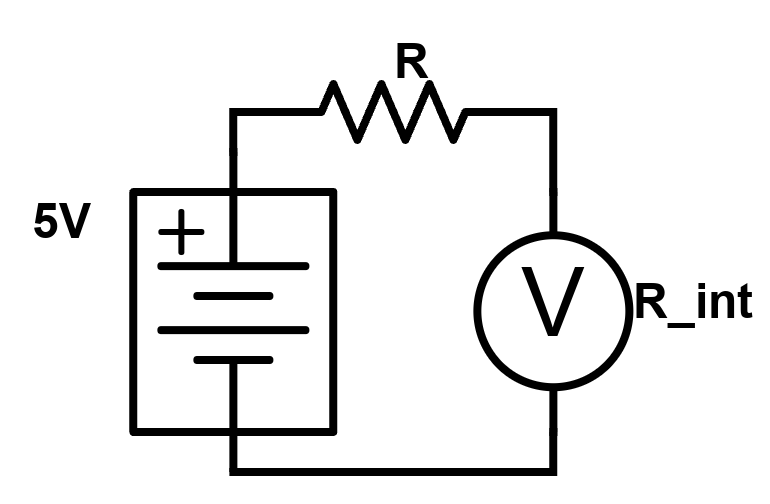
\includegraphics[width=0.4\linewidth]{vm.png}
        \caption{Internal Resistance of a Voltmeter}
    \end{figure}
    
    \begin{table}[H]
        \centering
        \begin{tabular}{c|c|c}
            \(R\) (\O)& \(V_m\) (V) & \(R_{int}\) (M\O)\\
            \hline
            1.19 & 5.00 & N/A\\
            10.5 & 5.00 & N/A\\
            1.51\(\times 10^8\) & 4.93  & 10.61 \\
            4.61\(\times 10^8\) & 4.78 & 10.02 \\
            8.29\(\times 10^{9}\) & 2.86 & 11.08 \\
            \hline
            Average & & 10.57 
        \end{tabular}
        \caption{Mastech Voltmeter Internal Resistance}
    \end{table}

    \begin{table}[H]
        \centering
        \begin{tabular}{c|c|c}
            \(R\) (\O) & \(V_m\) (V) & \(R_{int}\) (M\O)\\
            \hline
            \(1.51\times 10^{8}\) & 4.366 & 1.04\\
            \(2.20\times 10^{8}\) & 4.128 & 1.04\\
            \(3.30\times 10^{8}\) & 3.794 & 1.04\\
            \(5.71\times 10^{9}\) & 0.768 & 1.04\\
            \(9.95\times 10^{9}\) & 0.470 & 1.03\\
            \hline
            Average & & 1.04
        \end{tabular}
        \caption{Analog Discovery 2 Oscilliscope Internal Resistance}
    \end{table}

    In conclusion, the internal resistance of the Mastech voltmeter was measured to be \(10.57\) M\O. The internal resistance of the Active Discovery 2 oscilloscope was measured to be 1.04 M\O.

    \section{Ammeter Internal Resistance}

    After measuring the internal resistance of the two voltmeters we measured the internal resistance of the ammeter portion of the Mastech multimeter. Two resistors, \(R_0\) and \(R_1\) were connected in series and the ammeter was connected in parallel to \(R_1\). One resistor, \(R_0\) was chosen such that it was resistant enough to limit the overall current and prevent the resistors from being burnt out. The value of \(R_0\) was measured to be \(220.5\) \O. Next, the current through the circuit was measured with five different resistors in the place of \(R_1\). The resistance of each of these resistors was measured and recorded before being used in the circuit. The internal resistance was found by solving the system of equations 
    \begin{align*}
        I_1 + I_2 &= I_0\\
        5V - I_0\cdot R_0 - I_1\cdot R_1 &= 0\\
        I_2 \cdot R_{int} - I_1 \cdot R_1 &= 0
    \end{align*}
    for \(R_{int}\). This was done using row reduction on a matrix created from the known values. 
    \begin{table}[H]
        \centering
        \begin{tabular}[pos]{c|c|c}
            \(R_1\) (\O) & \(I_2\) (mA) & \(R_{int}\) (m\O)\\
            \hline
            1.41 & 1.68 & 22.6\\
            2.63 & 5.04 & 22.6\\
            5.24 & 9.31 & 22.6\\
            7.38 & 10.75 & 22.6\\
            10.69 & 13.10 & 22.6\\
            \hline
            Average & & 22.6
        \end{tabular}
        \caption{Mastech Ammeter Internal Resistance}
    \end{table}

    In conclusion, the internal resistance of the Mastech ammeter was measured to be \(22.6\) mA.

    \section{I-V Curves of Electrical Components}
    In the second part of the lab, we measured the I-V curves of LED lights, diodes, and a resistor. The plots for these are still in progress. 

    \section{Things I Learned}
    \begin{itemize}
        \item I had used a breadboard before but not very extensively, so I learned ways of keeping the circuit organized and how to make them easy to adjust in ways I know they will need to be adjusted. For example, placing a resistor in an easily accessible location because I know it will need to be swapped out.
        \item I learned how to navigate and use the Waveforms software.
        \item This lab also helped develop my intuition about how circuits work in general and the different effects that components in series or parallel can have. 
        \item I helped Audrey and Ryan on the bench behind mine with troubleshooting their circuits and also with using the Waveforms software. 
    \end{itemize}
\end{document}